\documentclass{ctexart}


\usepackage{cite}
\usepackage{graphicx}
\usepackage{tikz}
\usepackage{geometry}
\usepackage{url}
\usepackage{appendix}
\usepackage[colorlinks, linkcolor=black]{hyperref}
\geometry{left=3.17cm,right=3.17cm,top=2.54cm,bottom=2.54cm}
\usetikzlibrary{positioning, arrows.meta}

\tikzset{
  rect1/.style = {
    shape = rectangle,
    draw = white,
    text width = 1.2cm,
    rounded corners = 1mm,
    align = center,
    minimum height = 1cm,
  }
}
% 定义箭头样式
\tikzset{
  arrow1/.style = {
    draw = black, thick, -{Latex[length = 4mm, width = 1.5mm]},
  }
}



\title{Eigenfaces和Fisherfaces的比较与改进}
\date{\today}
\author{PB17111561-周恩帅 PB17111568-郭雨轩}

\begin{document}
    \maketitle

    \begin{abstract}
        本文给出了两种基于降维的人脸识别算法Eigenfaces和Fisherfaces的推导过程,同时对两种方法的进行了对比和改进。
        
        对于Eigenfaces算法,本文尝试从数据预处理、类内特征聚合和衡量类间差异的Metric三个维度对原有方法进行了改进,并在\texttt{Yale Faces B}数据集上定量的讨论这些改进各自产生的影响和联合产生的影响。
        我们发现在单独应用三种方法时,均可以使得算法精度提升;在联合使用时,也可以使得算法精度有较大提升。

        %% TODO:添加Fisherfaces摘要
        本论文的latex代码和实验用到的代码见此\href{https://github.com/SkilfulBugsMaker/Analysis-of-Eigenface-and-Fisherface}{github}仓库。
    \end{abstract}

    \tableofcontents
    \newpage
    

    \section{人脸识别算法的背景介绍}
    在这两种算法出现之前,大部分的人脸识别算法主要关注于识别特定的、单一的人脸特征,例如眼睛、鼻子、嘴或者脸的外轮廓。
    这些方法通过对上述特征出现的位置、形状大小以及相互的关系进行定义,最终得到一个人脸检测模型。
    但是它们有着非常明显的缺点,这些模型非常的脆弱,难以推广到多人脸、多视角的应用场景上去。
    
    在1987年,Sirovich和Kirby两人首次在他们的论文\cite{Sirovich:87}中证明了主成分分析(PCA)可以被用在图像集合上并得到一系列的“特征脸”,
    并且图像集合中的每一张脸都可以由这些“特征脸”线性组合重建出来,重建的误差会随着使用的“特征脸”的数目的增加而减少。

    Turk和A. Pentland于1991年在他们的论文\cite{doi:10.1162/jocn.1991.3.1.71}中给出了使用“特征脸”进行人脸识别的方法,这也是今天要介绍的Eigenfaces算法。
    在论文中,他们将人脸集合看成是一个由向量构成的集合,使用PCA的方法对人脸降维,再使用得到的“特征脸”计算出每张人脸的一个低维表示,使用这些低维表示,实现对人脸集合的分类。
    同时他们还介绍了一个快速求解维度很高的协方差矩阵的特征向量的方法,以便于快速得到人脸集合的“特征脸”。

    %% TODO:添加Fisherface的介绍

    \section{Eigenfaces和Fisherfaces算法数学推导}
    \subsection{Eigenfaces数学推导}
    \subsubsection{Eigenfaces 训练部分数学推导}
    在进行数学推导之前,需要说明的是,我们的目的是使用PCA的方法对输入的人脸数据集合进行降维,对于每张人脸得到一个低维表示,再根据这个低维表示对人脸数据进行分类。
    
    \noindent
    首先,对于输入的人脸图像集合把图像组织成列向量形式:
    $$
    \Gamma = \{\Gamma_1, \Gamma_2, \dots ,\Gamma_N \}
    $$
    之后,我们需要求出输入向量的平均值,即“平均脸”,可视化效果见附录图\ref{avg}:
    $$
    \Psi = \frac{1}{N}\sum_{i=1}^{N}\Gamma_i
    $$
    再根据“平均脸”求解出“误差脸”矩阵:
    $$
    \Phi_i = \Gamma_i - \Psi,\ A = \{ \Phi_1, \Phi_2,\dots,\Phi_N \}
    $$
    得到“误差脸”矩阵后,计算出协方差矩阵:
    $$
    C = AA^T
    $$
    该矩阵的$K$个特征向量即为所求的“特征脸”。为了求解这个矩阵的特征值和特征向量,我们需要对其使用SVD分解。
    值得注意的是,假定每张人脸图像的维度是$[w,h]$,那么每个人脸向量的维度也就是$[w\times h,1]$,则矩阵$C$的维度是$[w\times h,w \times h]$。
    在通常的图片中,$w \times h$的数量级一般在万级别或者十万级别,而对如此之大的一个矩阵做SVD分解的时间复杂度是非常大的。为了解决这个问题,
    我们可以先对这样一个小矩阵做SVD分解:
    $$
    C^* = A^TA
    $$
    这个矩阵的维度为$[N,N]$,其中$N$为人脸数据集的大小,在人脸识别的任务中,可以认为这个数量级是相对较小的。以一个典型的人脸数据集\texttt{Yale Face B}\cite{GeBeKr01}为例,$N=165$,而$w=320,h=243$,维度上的差距可以见得。
    我们对$C^*$矩阵求出特征向量$\vec{x_i}$:
    $$
    A^TA\vec{x_i} = \lambda_i \vec{x_i}
    $$
    再对上式左乘一个矩阵$A$,适当使用结合律,我们可以得到:
    $$
    (AA^T)(A\vec{x_i}) = C(A\vec{x_i}) = \lambda_i A \vec{x_i}
    $$
    可以看出,我们希望求得的矩阵$C$的特征向量$\vec{\mu_i}=A\vec{x_i}$,因此,我们可以先求出小矩阵$C^*$的特征向量$\vec{x_i}$,再对其特征向量左乘矩阵$A$,即得矩阵$C$的特征向量$\vec{\mu_i}$。
    至此,我们已经求得所有的"特征脸"$U=\{\mu_1, \mu_2,\dots,\mu_K \}$,可视化效果见附录图\ref{eigenface}。值得注意的是,矩阵$C$并不满秩,因为显然矩阵A中的每个列向量满足关系式:
    $$
    \sum_{i=1}^N\Phi_i = \sum_{i=1}^N(\Gamma_i-\Psi)=\sum_{i=1}^N\Gamma_i-N\cdot \frac{1}{N}\sum_{i=1}^N\Gamma_i=0
    $$
    即所有列向量是线性相关的。因此,矩阵$C$至多有$K-1$个有用的“特征脸”(对应的特征值不为0),可视化效果见附录图\ref{not-full-rank}。
    那么,我们求得的这些“特征脸”是否可以作为“脸空间”的标准正交基呢?答案是肯定的,由于矩阵$C=AA^T$是一个实对称矩阵,因而其所有的特征值都是正交的,我们只需要对求出的“特征脸”进行标准化,就可以得到一组“脸空间”的标准正交基,为了叙述方便,我们仍用$U$代指标准化后的“特征脸”。
    
    \noindent
    在得到了一组“脸空间”的基向量,也即“特征脸”之后,我们需要计算每一张已知的脸在这组基下的坐标$\Omega=[\omega_1, \omega_2, \dots, \omega_k]$。
    我们可以先考察对于一张特定的“误差脸”$\Phi_i$在一个特定的基$\vec{\mu_j}$上的投影,这就是$\omega^i_j$:
    $$
    \omega^i_j = \Phi_i^T \vec{\mu_j}
    $$
    那么一张脸的低维表示可以由以下公式给出:
    $$
    \Omega_i = \Phi_i^T U = [\omega_1^i, \omega_2^i, \dots, \omega_k^i]
    $$
    类似的,所有脸的低维表示可以由以下公式给出:
    $$
    \Omega = A^T U
    $$
    在实际操作中,对于一个类别的人脸,可能有多张人脸数据对应这一类,这时,这一类的低维表示被定义为:所有同属于这一类的人脸图像的低维表示的平均值。

    至此,基于PCA,我们已经对于每张输入的人脸数据都得到了一个低维表示,并且为每一类别生成了一个低维表示。
    \subsubsection{Eigenfaces 推断部分数学推导}

    这部分我将介绍如何使用训练部分生成低维表示对输入的图像进行人脸分类。

    \noindent
    对于每一张新输入的图片$\Gamma_{new}$,我们首先需要计算出它的“误差脸”$\Phi_{new}$:
    $$
    \Phi_{new} = \Gamma_{new} - \Psi
    $$
    之后,我们要计算出“误差脸”的低维表示$\Omega_{new}$:
    $$
    \Omega_{new} = \Phi_{new}^TU
    $$
    由上节的叙述,我们可以根据这个低维表示重建出输入的人脸$\Phi_{f}$:
    $$
    \Phi_f = \Omega_{new}U^T
    $$
    为了考察输入的图片是否为一张人脸图片,我们计算重建图像与原图像的误差$\epsilon_1$:
    $$
    \epsilon_1 = \|\Phi_{new}-\Phi_f\|^2
    $$
    如果误差过大,则认为不是一张人脸。排除掉输入图片是否为一张人脸的因素后,我们再将这个输入生成的低维表示与已知的每一类的低维计算误差,对于第$k$类的误差为$\epsilon^k_2$:
    $$
    \epsilon^k_2 = \| \Omega_{new} - \Omega_k \|^2
    $$
    当输入图像与某类的误差最小,且误差不超过预设的阈值时,我们可认为输入的人脸属于这一类,否则输入的人脸属于新的一类。

    \subsubsection{Eigenfaces 数学推导总结}
    \noindent
    综上,Eigenfaces的训练流程为:
    \begin{center}
        \begin{tikzpicture}
            \node[rect1, fill = green!20!white](1){输入训练人脸};
            \node[rect1, fill = green!20!white, right=of 1](2){计算平均脸};
            \node[rect1, fill = green!20!white, right=of 2](3){计算误差脸};
            \node[rect1, fill = green!20!white, right=of 3](4){计算特征脸};
            \node[rect1, fill = green!20!white, right=of 4](5){计算低维表示};
            \node[rect1, fill = green!20!white, right=of 5](6){为每类生成低维表示};
            \draw[arrow1](1) -- (2);
            \draw[arrow1](2) -- (3);
            \draw[arrow1](3) -- (4);
            \draw[arrow1](4) -- (5);
            \draw[arrow1](5) -- (6);
        \end{tikzpicture}
    \end{center}
    Eigenfaces的推断流程为:
    \begin{center}
        \begin{tikzpicture}
            \node[rect1, fill = pink!70!white](1){输入测试人脸};
            \node[rect1, fill = pink!70!white, right=of 1](2){计算误差脸};
            \node[rect1, fill = pink!70!white, right=of 2](3){计算与脸空间距离};
            \node[rect1, fill = pink!70!white, right=of 3](4){计算低维表示};
            \node[rect1, fill = pink!70!white, right=of 4](5){计算与每类误差};
            \node[rect1, fill = pink!70!white, right=of 5](6){判断人脸类别};
            \draw[arrow1](1) -- (2);
            \draw[arrow1](2) -- (3);
            \draw[arrow1](3) -- (4);
            \draw[arrow1](4) -- (5);
            \draw[arrow1](5) -- (6);
        \end{tikzpicture}
    \end{center}
    \subsection{Fisherfaces数学推导}
    %% TODO:添加Fisherfaces证明

    \section{两种算法的对比与改进措施}
    \subsection{两种算法的对比}
    %% TODO:对比两种算法的优缺点
    \subsection{对Eigenfaces的改进}
    \noindent
    对Eigenfaces的改进主要从以下三点出发,具体效果在实验部分展示:
    \begin{itemize}
        \item \textbf{数据预处理}:我们观察到数据集中同一类人脸的照片中出现了很多不同表情的照片,这些照片最主要的特点为人脸的上半部分基本相同,人脸的下半部分差异较大。
                因为对人脸分类不需要考虑其表情,所以我尝试去掉了下$1/3$人脸,仅保留剩余部分作为Eigenfaces的输入,数据可视化见附录图\ref{cropface}。
        \item \textbf{为每类生成低维度表示}:论文中为了生成每一类的低维表示,选择将同属于一类的低维表示取了平均值进行聚合。但是我们认为,取平均值可能会导致某些照片检测出现误差,
                我们尝试了不做任何聚合和在低维表示上的每个维度去做abs-max。
        \item \textbf{计算与每一类的误差}:在论文中使用的是$L_2\ loss$(也即MSE)作为评价的metric,它对低维表示中的离群维度比较敏感。
                但是在这个场景中,可能仅仅需要要求大部分维度的低维表示接近时我们就可以断定输入图像属于这一类,基于此我们尝试了$L_1\ loss$(也即MAE)作为评价的metric;
                还有可能仅仅需要输入图像的低维表示的方向与对应类别的低维表示接近即可,基于这个想法我们也尝试了$cosine\ loss$(也即余弦相似度)作为评价的metric。
    \end{itemize}

    \subsection{对Fisherfaces的改进}
    %% TODO:添加对Fisherfaces的改进(如果有的话)


    \section{实验部分}
    我们使用\texttt{Yale Faces B}\cite{GeBeKr01}数据集对两种方法及改进分别进行了测试,这个数据集包含165张人脸图片,一共有15个类别,每类有11张灰度图片,分辨率为$320\times 243$,包含同一个人在不同光照条件下和不同表情下的图片,部分数据集图片如下:
    \begin{figure}[htbp]
        \centering
        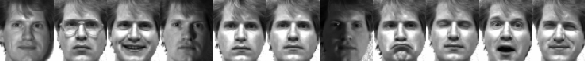
\includegraphics[scale=0.7]{imgs/yale-face-B.png}
        \caption{\texttt{Yale Face B}数据集}
    \end{figure}
    \subsection{Eigenface 实验}
    
    \begin{figure}[htbp]
        \begin{minipage}[t]{0.45 \linewidth}
            \centering
            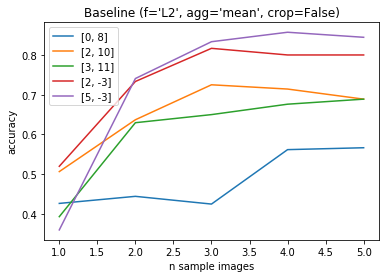
\includegraphics[scale=0.45]{imgs/baseline.png}
            \caption{基准模型}
            \label{baseline}
        \end{minipage}
        \begin{minipage}[t]{0.45 \linewidth}
            \centering
            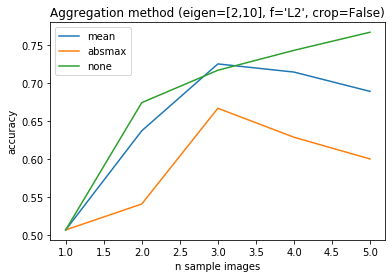
\includegraphics[scale=0.45]{imgs/agg.png}
            \caption{改变特征聚合方式的模型}
            \label{agg}
        \end{minipage}
    \end{figure}
    首先我们测试了在不同采样率和不同的“特征脸”选取策略下的精度,见图\ref{baseline},这张图的横坐标为每种类采样的图片数量,纵坐标为准确率,不同的曲线为不同的特征向量的选取策略。
    例如$[0,8]$表示选取第1大到第8大的特征向量作为“脸空间”的基,$[2,-3]$代表选取第3大到倒数第3大的特征向量作为“脸空间”的基。图中可以明显的看出,当使用了特征值比较大的特征向量时,
    精度反而较低,根据Eigenfaces论文\cite{doi:10.1162/jocn.1991.3.1.71}论文中的说法,Eigenfaces是一个对光照敏感的模型,而特征值较大的特征向量会包含光照的信息,导致结果准确率较低。
    我们也可以看到当“脸空间”的特征向量的数目增加时,精确率会有明显的上升,这是因为越多的特征向量会有更好的重建性能,但是同时也会导致更大的计算开销。在我们后续的对比试验中,
    我们固定特征向量选取策略为$[2,10]$,这是一个有着不错效果,同时又不会导致很大的计算开销的策略,来横向对比不同的改进措施产生的影响。
    
    然后我们测试了在不同采样率和不同的类内特征聚合方式的模型,它与基准模型仅在聚合的方式上有所不同,见图\ref{agg}。可以看出,在不同采样率上,不聚合的方式较于基准模型有着更优的精度,二者都好于使用abs-max的方式。
    这可能是因为,对同属一类的低维表示使用平均值可能会导致信息损失,不进行聚合可以保证更好的多样性,但是也会带来更大的存储开销;abs-max的方式效果较差,可能是因为在用$L_2\ loss$衡量输入与每一类误差的时候会导致得到的结果与预期偏差更大,从而使得精度下降。
    \begin{figure}[htbp]
        \begin{minipage}[t]{0.45 \linewidth}
            \centering
            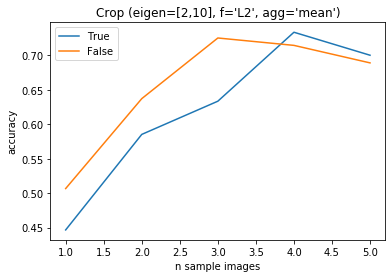
\includegraphics[scale=0.45]{imgs/crop.png}
            \caption{对输入数据预处理的模型}
            \label{crop}
        \end{minipage}
        \begin{minipage}[t]{0.45 \linewidth}
            \centering
            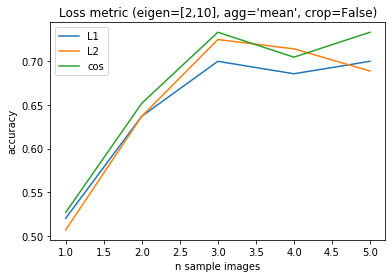
\includegraphics[scale=0.45]{imgs/loss-metric.png}
            \caption{改变损失指标的模型}
            \label{loss}
        \end{minipage}
    \end{figure}
    
    接下来我们测试了仅进行预处理(对图片裁切到下$1/3$)带来的影响,见图\ref{crop}。可以看到,当采样率较大的时候,进行预处理的效果要比不进行预处理的效果要好,这可能是因为当采样率增大,加上使用平均作为类内特征聚合的方式,会导致训练集中差异较大的部分被平均化,导致测试集中的每张图片都与正确类别的低维表示差距较大,
    而进行裁切后,去掉了差异化较大的部分,仅保留了共性的部分,因此图像更容易被判别到正确的类别。

    之后我们测试了仅改变衡量类归属的指标带来的影响,见图\ref{loss}。基准模型使用的是$L_2 \ loss$,当采样率增大的时候$L_1 \ loss$和$cosine \ loss$的效果均高于基准模型,这可能是因为,$L_2 \ loss$更加关注低维表示中的离群维度,而随着采样率的增大,训练集数据间的差异也在增大,
    导致即使属于同一类的低维表示,在这个向量的某一维也可能有较大的差距,而使用$L_2 \ loss$则放大了这个差距,导致精度下降,另外两种没有这种情况。

    \begin{figure}[htbp]
        \centering
        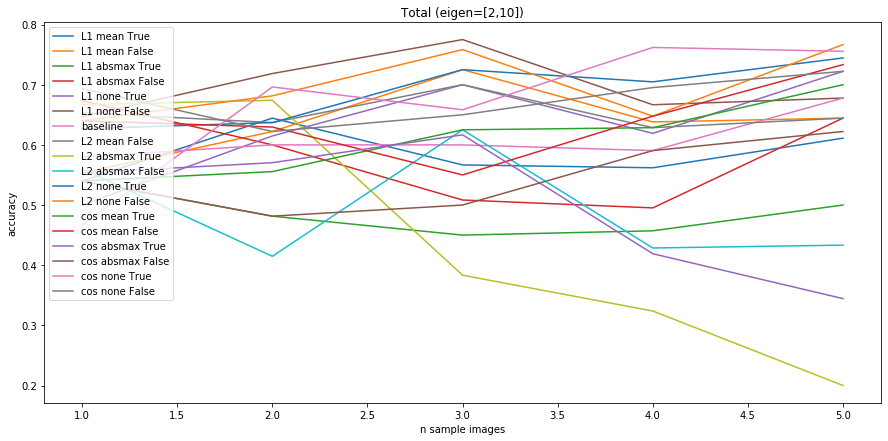
\includegraphics[scale=0.45]{imgs/total1.png}
        \caption{选取$[2,10]$特征向量,三种策略联合}
        \label{total1}
    \end{figure}
    \begin{figure}[htbp]
        \centering
        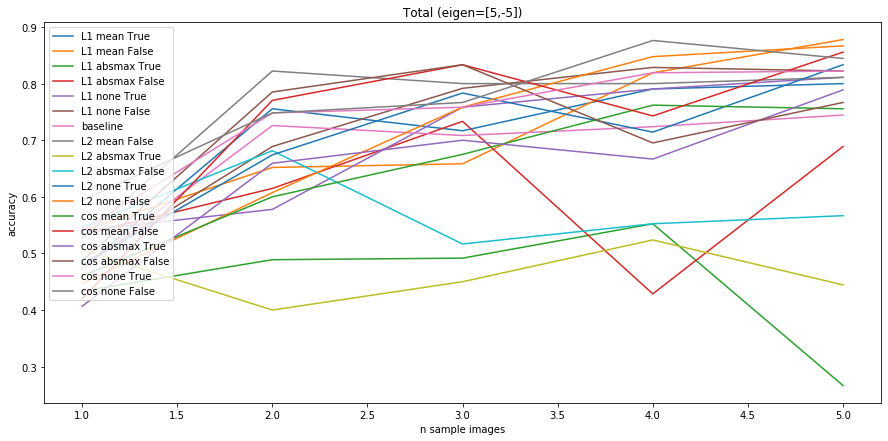
\includegraphics[scale=0.45]{imgs/total2.png}
        \caption{选取$[5,-5]$特征向量,三种策略联合}
        \label{total2}
    \end{figure}

    最后我们将测试了三种方式联合使用时产生的影响,见图\ref{total1}和图\ref{total2}。两图的主要差别在特征向量的选取策略不同,前者可以认为是在受限的特征向量的选取场景下,后者可认为是在理想情况下。
    可以看到当联合使用三种改进方式时,有部分排列组合相较于基准模型有了较大的提升,说明所提出的三种模型在改进的方向上是相对较为独立的,都各自解决了部分Eigenfaces模型原有的一些不足。


    \subsection{Fisherfaces 实验}
    %% TODO:补充Fisherfaces的实验

    \section{结论}
    对于两种算法,本文分别给出了它们的数学推导
    对于Eigenfaces算法,本文从三个维度尝试对其改进,独立应用时均有小幅度精度提升,在联合使用时也有明显的精度提升。
    %% TODO:宁再随便扯两句Fisherfaces的结论和两种方法比较的结论
    

    \newpage
    \addcontentsline{toc}{section}{参考文献}
    \bibliographystyle{plain}
    \bibliography{ref}

    \newpage
    \appendix
    \section{附录}
    在这部分我们给出Eigenface的部分中间结果的可视化效果。
    \begin{figure}[htbp]
        \begin{minipage}[t]{0.45 \linewidth}
            \centering
            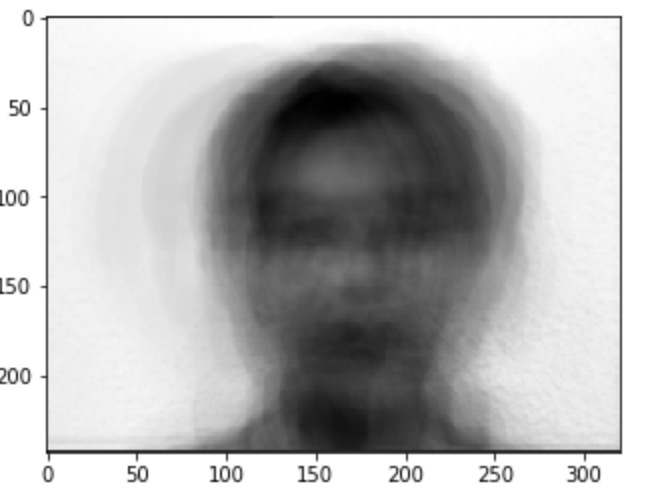
\includegraphics[scale=0.23]{imgs/avg_face.png}
            \caption{平均脸}
            \label{avg}
        \end{minipage}
        \begin{minipage}[t]{0.45 \linewidth}
            \centering
            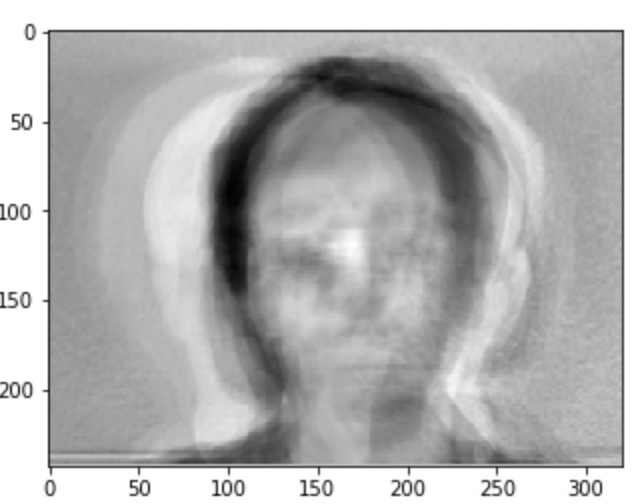
\includegraphics[scale=0.45]{imgs/eigenface.png}
            \caption{特征脸}
            \label{eigenface}
        \end{minipage}
    \end{figure}
    \begin{figure}[htbp]
        \begin{minipage}[t]{0.45 \linewidth}
            \centering
            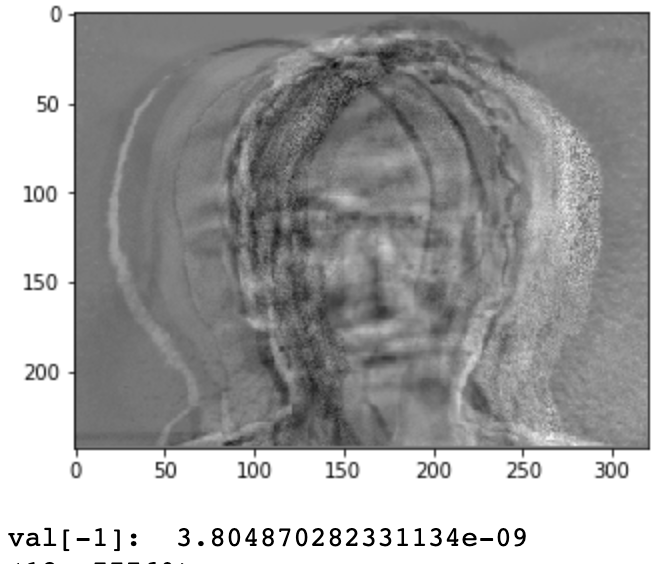
\includegraphics[scale=0.45]{imgs/not-full-rank.png}
            \caption{最后一个特征脸及其对应的特征值}
            \label{not-full-rank}
            \end{minipage}
        \begin{minipage}[t]{0.45 \linewidth}
            \centering
            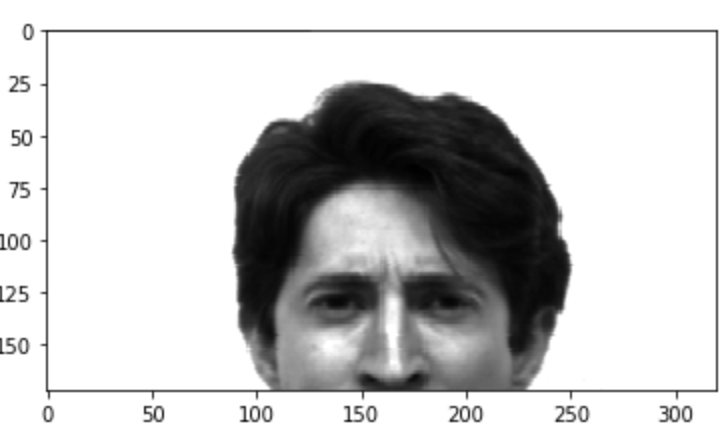
\includegraphics[scale=0.45]{imgs/semi_face.png}
            \caption{裁切脸}
            \label{cropface}
        \end{minipage}
    \end{figure}

\end{document}